\subsection{Integrated anonymous download}
An substantial effort was made to integrated the tunnel community and hidden services community with the MultiChain community.
These communities work together to provide functionality to transfer data anonymously.
The tunnel community reports data transferred between peers and the MultiChain community add these amounts to the chain.
They are already integrated with BarterCast.
The method of integration of BarterCast was used to try to integrated MultiChain aswell.
Setting up the Gumby environment to run all communities took also considerable time.

Experiments were conducted where an 100 MB file is transferred by the actual anonymity communities,
while MultiChain transcribes the transfer amounts in the MultiChain.
The amount of hops is varied between 0 and 2.
The result of these experiments show that the integration was not done properly.
There are two problems that were identified using the results of the experiments.

When the experiment is conducted without any hops,
the integration does not report any data transferred between the peers.
As such the scheduler never sees a reason to schedule a signature request.
The whole MultiChain community is never active.
The connection between the seeder and the first hop,
or the downloader, directly is not reported to the scheduler.

Secondly, there is a problem in the data that is reported by the data that is sent by hops.
Too much data is reported and it is unclear where this data originates from.
The overhead measures twice the actual download size.
The results can be seen in Figure \ref{fig:integrated-anonymous-amounts}.

\begin{figure}
\centering
\subfigure[Total download amount.]{
\centerline{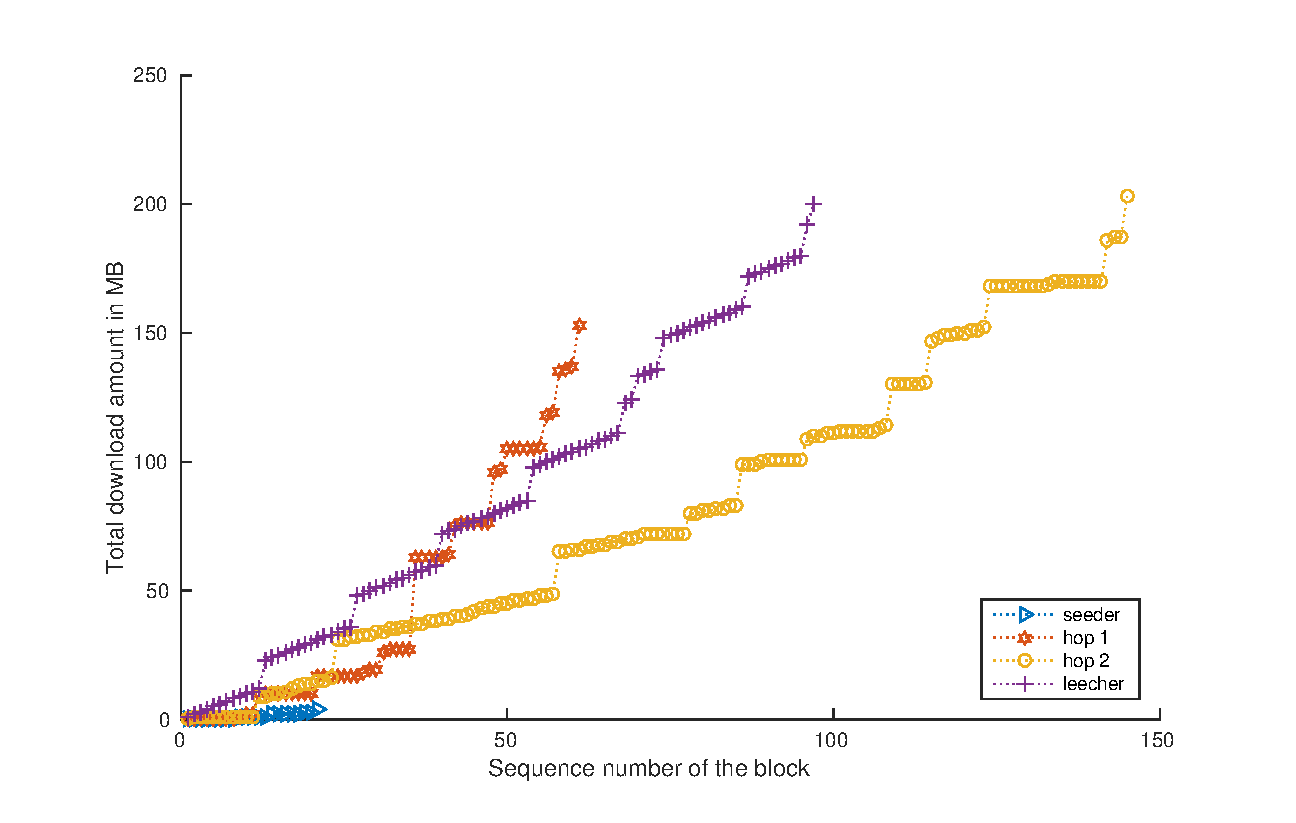
\includegraphics[scale=0.5]{experimentation/anonymous-integrated/integrated-anonymous-down.eps}}
\label{fig:integrated-anonymous-down}
}
\subfigure[Total upload amount.]{
\centerline{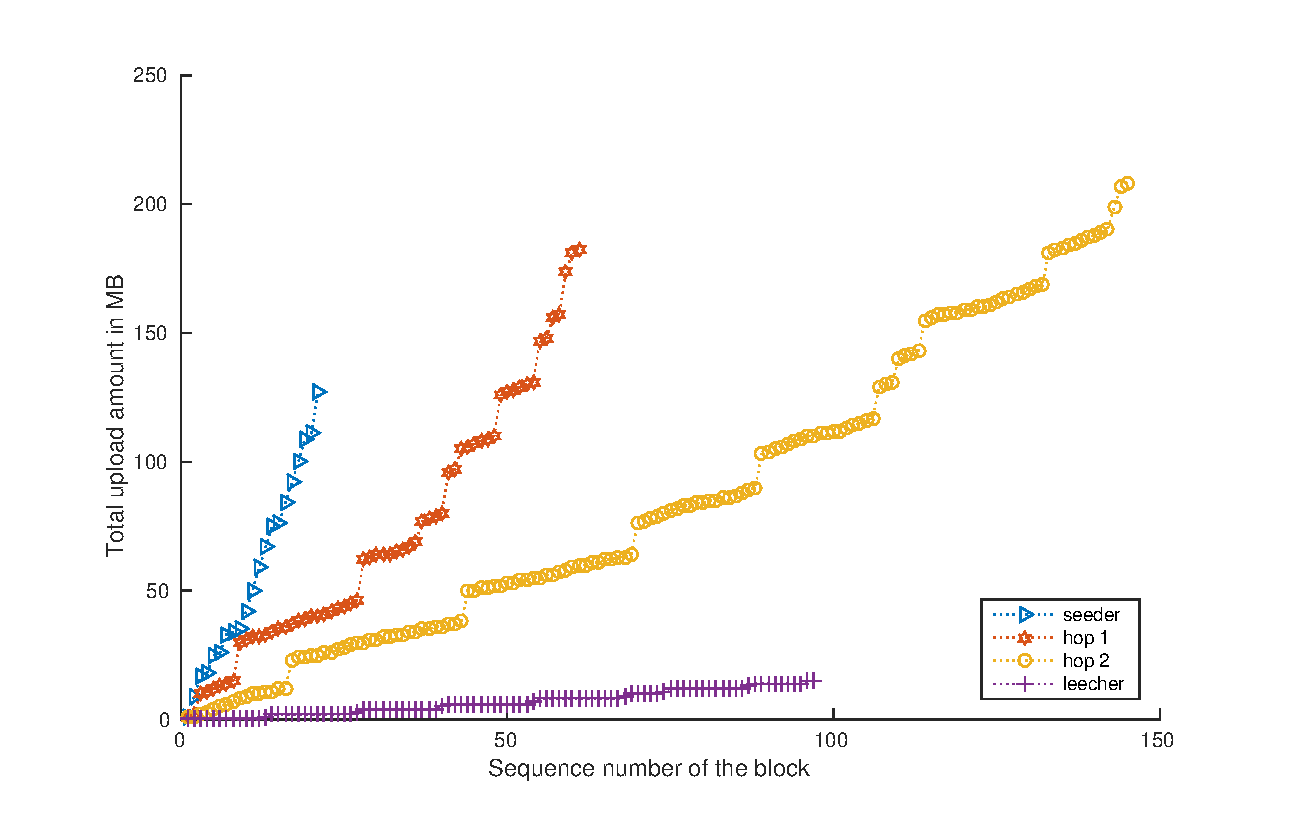
\includegraphics[scale=0.5]{experimentation/anonymous-integrated/integrated-anonymous-up.eps}}
\label{fig:integrated-anonymous-up}
}
\caption{Download and upload amounts during the integrated anonymous download experiment.}
\label{fig:integrated-anonymous-amounts}
\end{figure}